\section{State of the art: $\mathcal{H}$ to $\mathcal{V}$}
\AtBeginSection[]
  {
     \begin{frame}<beamer>
     \frametitle{Plan}
     \tableofcontents[currentsection]
     \end{frame}
  }
\subsection{The simplex algorithm}

\begin{frame}{Linear optimization problems}
\begin{block}{Assumptions}
\begin{itemize}
\item $0$ is in the intersection.
\item All the variables are positive.
\end{itemize}
\end{block}
\begin{figure}
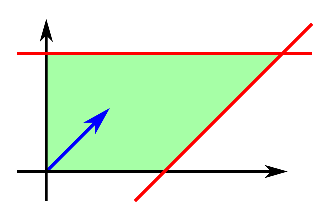
\includegraphics[scale=1]{images/simplex1.eps}\\
Example of linear optimization problem with the objective $x+y$ and the constraints $y\leq 1$ and $x-y\leq 1$.
\end{figure}
\end{frame}

\begin{frame}{The simplex}
\begin{theorem}
For a problem in $\mathbb{R}^d$, the optimal is either unbounded or reached by the intersection of $d$ independent hyperplanes.
\end{theorem}


\begin{figure}
\only<1>{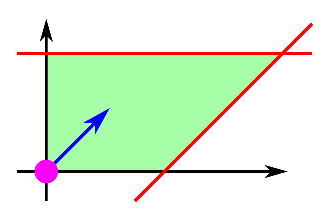
\includegraphics[scale=1]{images/simplex12.eps}}
\only<2>{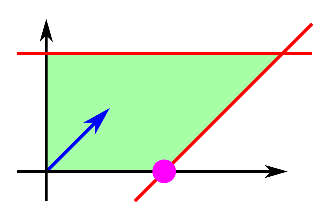
\includegraphics[scale=1]{images/simplex13.eps}}
\only<3>{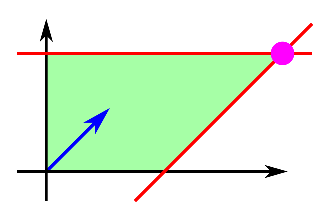
\includegraphics[scale=1]{images/simplex14.eps}}

The simplex algorithm on the previous example.
\end{figure}  

\end{frame}

\begin{frame}{The dictionary}
\begin{block}{Construction of the slack variables}
$-x+y\leq 3 \hspace*{1cm} \rightarrow \hspace*{1cm} 0 \leq x - y + 3 \hspace*{1cm} \rightarrow \hspace*{1cm} 0\leq s_1 = x - y + 3$
\end{block}
The dictionary keeps track of all the constrains.
\begin{block}{Construction of the dictionary}
\begin{tabular}{| c  c  c  c  c | c c |}
	\hline	
   	$-x$ &$+$& $0$ & $+$ & $2$ & = & $s_1$\\ \hline	
   	$x$ &$+$& $-y$ & $+$ & $3$ & = & $s_2$\\ \hline \hline	
   	$x$ & $+$ & $y$ & & & &  \\
   	\hline	
\end{tabular}
$\rightarrow$
\begin{tabular}{| c | c || c || c c |}
	\hline	
	$x$ & $y$ & const & & \\
	$\downarrow$ &$\downarrow$ &$\downarrow$ & & \\
	\hline
	\hline	
   	$-1$ & $0$ & $2$ & = & $s_1$\\ \hline	
   	$1$ & $-1$ & $3$ & = & $s_2$\\ \hline \hline	
   	$1$ & $1$ & $0$ & $\leftarrow$ & obj \\
   	\hline	
\end{tabular}

\end{block}

\end{frame}

\begin{frame}{Some properties}
\begin{table}
\centering
\begin{tabular}{| c | c || c || c c | c}
	\multicolumn{4}{l}{Cobasis} & \multicolumn{2}{l}{ }\\
	\cline{1-5}	
	$x$ & $y$ & const & & & \\
	$\downarrow$ &$\downarrow$ &$\downarrow$ & & & \\
	\cline{1-5}
	\cline{1-5}	
   	$-1$ & $0$ & $2$ & = & $s_1$ & \multirow{2}{*}{\rotatebox{270}{\hspace*{-0.4cm} Basis}} \\ \cline{1-5}	
   	$1$ & $-1$ & $3$ & = & $s_2$ \\ \cline{1-5} \cline{1-5}	
   	$1$ & $1$ & $0$ & $\leftarrow$ & obj & \\
   	\cline{1-5}
\end{tabular}
\end{table}
\vspace*{0.5cm}
\begin{itemize}
\item The cobasis gives the value of the basis.
\item The variables of the cobasis are independent.
\item The dictionary describes the vertex.
\end{itemize}

Only one operation: the pivot.
\end{frame}

%\begin{frame}{Other version of the simplex}
%If there are non positive variables or if $0$ is not in the feasible area.
%\begin{itemize}
%\item For each variable, keep lower and upper bounds, plus a valuation.
%\item While there is a basic variable out of it bounds, pivot with a variable that can increase/decrease and modify the assignment.
%\item Optimize.
%\end{itemize}

%\begin{figure}
%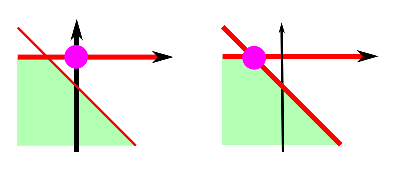
\includegraphics[scale=1]{images/simplex2.eps}
%\caption{Example of the other version of the simplex with $y\leq 0$ and $x+y\leq -1$.}
%\end{figure}
%\end{frame}

\subsection{Fukuda's algorithm}



\begin{frame}{An example}
\begin{figure}
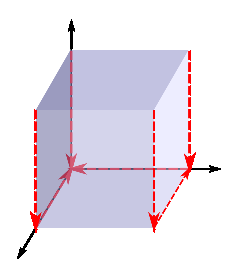
\includegraphics[width=0.35\columnwidth]{images/fukuda.eps}

\includegraphics[width=0.35\columnwidth]{images/fukugraph.eps}

For the unit cube in $\mathbb{R}^3$, the different paths to reach the origin and the tree of Fukuda's research.
\end{figure}
\end{frame}



\begin{frame}{Fukuda's algorithm}
Enumerates the vertices of a bounded $\mathcal{H}$-polyhedron. 

\begin{block}{Main idea}
Reversed simplex for a function maximizing only the origin.
\end{block}

\begin{itemize}
\item All the vertices are found.
\item If there exist several ways of defining a vertex, all the ways will be found.
\end{itemize}
\end{frame}



\begin{frame}{An example}
Fukuda's Algorithm with the constraint $ x+2y \leq 4 $.
\begin{columns}[c]
\begin{column}{5cm}
\only<1,3>{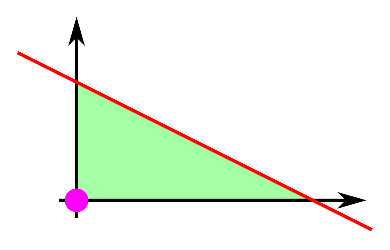
\includegraphics[scale=0.9]{images/fukuda0.eps}}
\only<2>{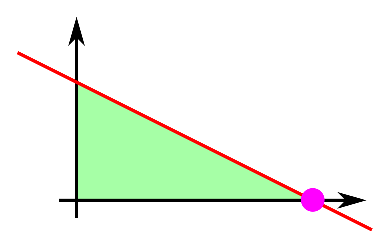
\includegraphics[scale=0.9]{images/fukuda1.eps}}
\only<4>{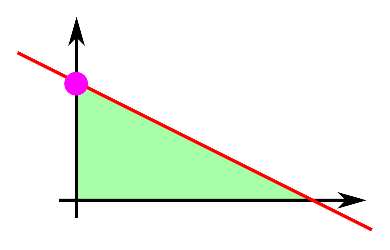
\includegraphics[scale=0.9]{images/fukuda2.eps}}
\end{column}
\begin{column}{5cm}


\only<1,2>{
\begin{tabular}{| c | c || c || c c |}
	\hline	
	$x$ & $y$ & const & & \\
	$\downarrow$ &$\downarrow$ &$\downarrow$ & & \\
	\hline
	\hline	
   	$-1$ & $-2$ & $4$ & = & $s_1$\\ \hline \hline	
   	$-1$ & $-1$ & $0$ & $\leftarrow$ & obj \\
   	\hline	
\end{tabular}

\vspace*{0.3cm}


\visible<2>{\begin{tabular}{| c | c || c || c c |}
	\hline	
	\textcolor{red}{$s_1$} & $y$ & const & & \\
	$\downarrow$ &$\downarrow$ &$\downarrow$ & & \\
	\hline
	\hline	
   	$-1$ & $-2$ & $4$ & = & \textcolor{red}{$x$}\\ \hline \hline	
   	$1$ & $1$ & $-4$ & $\leftarrow$ & obj \\
   	\hline	
\end{tabular}
}}
\only<3,4>{
\begin{tabular}{| c | c || c || c c |}
	\hline	
	$x$ & $y$ & const & & \\
	$\downarrow$ &$\downarrow$ &$\downarrow$ & & \\
	\hline
	\hline	
   	$-1$ & $-2$ & $4$ & = & $s_1$\\ \hline \hline	
   	$-1$ & $-1$ & $0$ & $\leftarrow$ & obj \\
   	\hline	
\end{tabular}

\vspace*{0.3cm}

\visible<4>{\begin{tabular}{| c | c || c || c c |}
	\hline	
	$x$ & $\textcolor{red}{s_1}$ & const & & \\
	$\downarrow$ &$\downarrow$ &$\downarrow$ & & \\
	\hline
	\hline	
   	$-\frac{1}{2}$ & $-\frac{1}{2}$ & $2$ & = & \textcolor{red}{$y$}\\ \hline \hline	
   	$-\frac{3}{2}$ & $\frac{1}{2}$ & $-2$ & $\leftarrow$ & obj \\
   	\hline	
\end{tabular}}
}
\end{column}
\end{columns}
\end{frame}
